\section{Kings: Certificates, Loopy Games and the Failure Sweep}\label{S-kings}
This section holds the parts of Section~\ref{sec:kings} of the main text that were moved out: the certificate theory, the local test for (V2), the loopy games and the details of the failure sweep. Full proofs are in Section~\ref{S-kingsproof}.
\subsection{Certificates}
A local test for (V3) is the \emph{certificate of horizon $h$} of a move in $Z$. Let the punisher answer with a move in $Z$ that does not promote and leaves its king among
the files of $Z$, and call the position then reached $Q$, with the defender to move. (i) With all pawns outside $Z$ removed, the punisher wins the local game: whatever the defender does, and
even if it may pass whenever it is not in check, the punisher (who never passes) promotes or mates with one of its first $h$ moves counted from $Q$, and the defender promotes first
in no play. (ii) With the punisher's king and all pawns in $Z$ removed, and the defender alone to move, no sequence of defender king and pawn moves ends in a promotion within $h$
moves (a king may capture, never steps onto a square attacked by a punisher pawn, and the punisher's other pawns stand still); the defender's pawns in $Z$ fall under (i) (the \emph{counter-promotion condition}). (iii)
The punisher can follow its winning strategy of (i) so that in no play is the defender stalemated before the punisher's $h$-th move. It works in the \emph{promotion game}, where the first promotion wins.

\begin{theorem}[\lab{S}]\label{thm:cert}
In the promotion game, a move in $Z$ with a certificate of horizon $h$ is a loss for its mover, so the
promotion-game analogue of (V3) holds if every move in $Z$, at every position before the first decisive event, has one; for chess, (V3) needs the further
check that a won promotion race is a won game. Clause (ii) cannot be weakened to $h-1$ moves \lab{C1}.
\end{theorem}

In chess small margins fail. On the cylinder with seven files and six ranks, Kb4, Pe4 against Ka1, Pa2 with
white to move, the king move Kb4--c5 has a certificate of horizon~1, yet the chess result after it is a draw, and
Kc5--d5 in Kc5, Pe2 against Ka3, Pc4 on the same board has horizon~2, yet White wins \lab{C1}.

For (V2) we give a sufficient test in the frozen-king game \lab{S} (Proposition~A.19 of Section~\ref{S-kingslong}): the side credited
after a context move that makes a passed pawn wins that game if it has an e.p.-aware passed pawn with a clear
path, the king-safety, escape-square and nearby-pawn conditions of Proposition~A.19 hold, and, with this pawn
removed, no sequence of enemy pawn moves promotes within the enemy turns available before its promoting push. The model looks only at passed pawns: with Pc2, Pd4 against
Pd3 on the $8\times6$ cylinder, black to move, it credits white, yet d3$\times$c2 and c1=Q come first \lab{C1}.

\begin{proposition}[\lab{S}]\label{prop:horizon1}
On boards with at least six ranks, for $h=1$, the counter-promotion condition holds in every chess-legal
context without a passed pawn.
\end{proposition}

\begin{proof}
A pawn that can promote in one move stands on the rank before its last. With six or more ranks it got there by a
single step or a capture, so it cannot be taken en passant, and no enemy pawn can stand ahead of it: it is
already passed.
\end{proof}

\begin{conjecture}[\lab{Conj}]\label{conj:horizon2}
On a board with room for two files beyond the buffer, for every king group whose punishment needs $h\ge2$
moves, some context without a passed pawn leaves a move in the group unpunished.
\end{conjecture}

Real tr\'ebuchets seem to need $h\approx5$--$7$ \lab{Conj}, and a locked pawn pair can still break their zero \lab{C2}. An example: the tr\'ebuchet \pos{W Ka4 b3 / B Kc3 b4} on the cylinder with seven files and six ranks acts as zero in the promotion game beside the locked pair \pos{W e3 / B e4}, but beside the locked pair \pos{W e2 / B e3}, which also has no move and no passed pawn, black to move wins by 1\dots Kd2 instead of losing. Three separately written programs agree; no hand proof is given.

\subsection{Spare King Moves Are Loopy}

A king that can step back and forth without loss gives its side unlimited waiting moves, a loopy
game~\cite{WinningWays,Siegel2013}: $\textsf{on}=\game{\textsf{on}}{}$ if only white can wait,
$\textsf{off}=-\textsf{on}$ if only black can, and $\textsf{dud}$ if both can. Since $\textsf{on}$ exceeds every number, $\BIG$ included, the $\pm\BIG$ convention fails there, and a
decisive event must instead end the game.

\begin{theorem}[Outcomes with spare moves; \lab{S}]\label{thm:loopy}
Let the components form a short game in which every decisive event ends the game, let a side that can wait pass
at any time, and let every other move in $Z$ lose. If only white can wait, black wins exactly when it can force a decisive
event in its favor against a passing white, and white wins otherwise. If both can wait, a side wins exactly when
it can do so against a passing opponent, and otherwise the game is drawn.
\end{theorem}

\begin{proof}[Proof sketch]
If only white can wait, every play is finite, since black's moves are, so the game is determined, and black
wins exactly when some move of black's wins against every white reply, a pass included. If both can wait, a
winning side never needs to pass, so it wins exactly when it can force a decisive event against passes;
otherwise play can go on forever. The full proof is Theorem~A.18a of Section~\ref{S-kingslong}.
\end{proof}

Beside a spare king move, then, component values matter only through their forcing threats. The kings
alone are already loopy: in normal play (a stalemate loses), every quiet K+P against K placement on the boards
from $3\times4$ to $5\times5$, summed with sixteen test games, behaves as a decisive win, $\textsf{on}$,
$\textsf{off}$ or $\textsf{dud}$, or as none of these; none behaves as a number or an infinitesimal, and removing
the edges changes the class of $12.5$--$20.5\%$ of them \lab{C2} (the counts are in \texttt{kings/REPORT.md}, task K4, in the code copy).

\subsection{Details of the Failure Sweep}
We solved, with the kings played out, every component with at most two pawns a side beside a
tr\'ebuchet on boards with six ranks: on one file of the six-file cylinder and of the five-file ordinary board,
and on files d and e of the seven-file cylinder (queen promotions only, at most two queens at a time). Of these, $500$ start without a race and have a determined result. Under the textbook test, $159$ of the $500$ get the wrong outcome \lab{C1}: $107$ through
the kings alone, $18$ through en passant and $34$ because a passed pawn does not win its race. $143$ of the
$159$ are on the seven-file cylinder. The e.p.-aware test repairs the $18$ e.p.\ failures, but the kings undo $13$ of these repairs. On the ordinary $8\times8$ board, in $94$ positions beside a tr\'ebuchet checked against the tablebase, the
convention says all $449$ king moves lose, yet $41$ draw and $7$ win \lab{C1}. The $34$ race failures have one cause: a blocked
enemy pawn steps level with its blocker and promotes first. Ending the game only at a passer that wins the
race by the square rule removes all $52$ convention failures with frozen kings; with real kings $31$ stay repaired, which leaves $128$ mismatches, all from the
kings \lab{C1}. The rule is not sound on every board: on three files, \pos{W a4 b6 / B c7} with black to move passes it, yet black wins. Of the $2{,}154$ $8\times8$ positions beside a tr\'ebuchet whose real results we could compute (not a random sample), $105$ are
draws; in the other $2{,}049$ the model names the winner in $92.5\%$, against $83\%$ and $84\%$ under the mover
and opponent rules \lab{C1}. These positions are the ones our other runs solved, not a sample of a defined class.

Fig.~\ref{fig:f3} shows the agreement rates with Wilson 95\% intervals. The intervals treat positions as independent and so are optimistic.
\begin{figure}[!htbp]
\centering
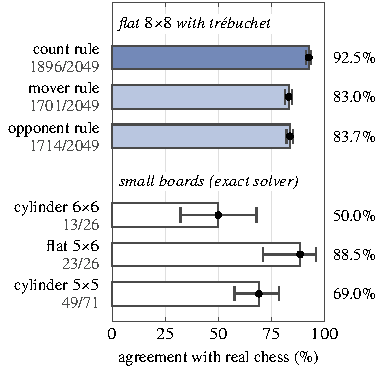
\includegraphics{figures/f3_model_vs_chess.pdf}
\caption{Agreement between the model and real chess, with Wilson 95\% intervals. Top: ordinary $8\times8$ board
beside a tr\'ebuchet, $2{,}049$ decisive positions, by race rule (count rule best). Bottom: exact king-and-pawn
results on small boards.}
\label{fig:f3}
\end{figure}
